\documentclass[11pt,a4paper,twoside,openright]{report}

\usepackage[top=25mm,bottom=25mm,right=25mm,left=30mm,head=12.5mm,foot=12.5mm]{geometry}
\let\openright=\cleardoublepage

\usepackage[a-2u]{pdfx}
\catcode30=12

\usepackage[
   backend=biber
%  ,style=iso-authoryear
  ,style=numeric
  ,citestyle=numeric
  ,sortlocale=cs_CZ
  ,bibencoding=UTF8
  %,block=ragged
]{biblatex}
\addbibresource{references.bib}

%% Přepneme na českou sazbu, fonty Latin Modern a kódování češtiny
\usepackage[czech]{babel}
\usepackage{lmodern}
\usepackage[T1]{fontenc}
\usepackage{textcomp}
\usepackage[utf8]{inputenc}

% Set fonts
\RequirePackage[osf]{mathpazo} % Palatino with oldstyle figures
\newcommand\liningnums[1]{\fontfamily{ppl}\selectfont#1}
\RequirePackage{eulervm}
\RequirePackage[scaled=.8819]{sourcecodepro} % Source Code Pro typeface for monospace

%%% Další užitečné balíčky (jsou součástí běžných distribucí LaTeXu)
\usepackage{amsmath}        % rozšíření pro sazbu matematiky
\usepackage{amsfonts}       % matematické fonty
\usepackage{amsthm}         % sazba vět, definic apod.
\usepackage{bm}             % tučné symboly (příkaz \bm)
\usepackage{graphicx}       % vkládání obrázků
\usepackage{fancyvrb}       % vylepšené prostředí pro strojové písmo
\usepackage{fancyhdr}       % prostředí pohodlnější nastavení hlavy a paty stránek
\usepackage{icomma}         % inteligetní čárka v matematickém módu
\usepackage{dcolumn}        % lepší zarovnání sloupců v tabulkách
\usepackage{booktabs}       % lepší vodorovné linky v tabulkách
\makeatletter
\@ifpackageloaded{xcolor}{
   \@ifpackagewith{xcolor}{usenames}{}{\PassOptionsToPackage{usenames}{xcolor}}
  }{\usepackage[usenames]{xcolor}} % barevná sazba
\makeatother
\usepackage{multicol}       % práce s více sloupci na stránce
\usepackage{caption}
\usepackage{enumitem}
\usepackage{lipsum}
\usepackage{wrapfig}
\setlist[itemize]{noitemsep, topsep=0pt, partopsep=0pt}
\setlist[enumerate]{noitemsep, topsep=0pt, partopsep=0pt}
\setlist[description]{noitemsep, topsep=0pt, partopsep=0pt}
\usepackage{pdfpages}

\usepackage{tocloft}
\setlength\cftparskip{0pt}
\setlength\cftbeforechapskip{1.5ex}
\setlength\cftfigindent{0pt}
\setlength\cfttabindent{0pt}
\setlength\cftbeforeloftitleskip{0pt}
\setlength\cftbeforelottitleskip{0pt}
\setlength\cftbeforetoctitleskip{0pt}
\renewcommand{\cftlottitlefont}{\Huge\bfseries}
\renewcommand{\cftloftitlefont}{\Huge\bfseries}
\renewcommand{\cfttoctitlefont}{\Huge\bfseries}

% vyznaceni odstavcu
\parindent=0pt
\parskip=11pt

% zakaz vdov a sirotku - jednoradkovych pocatku ci koncu odstavcu na prechodu mezi strankami
\clubpenalty=1000
\widowpenalty=1000
\displaywidowpenalty=1000

% nastaveni radkovani
\renewcommand{\baselinestretch}{1.20}

% nastavení hlavy a paty stránek
\fancyhf{}
\renewcommand{\chaptermark}[1]{\markboth{#1}{}}
\fancyhead[RO,LE]{\leftmark}
\fancyfoot[RO,LE]{\thepage}
%\renewcommand{\footrulewidth}{0pt}
\fancypagestyle{plain}{%
\fancyhf{} % clear all header and footer fields
\fancyfoot[RO,LE]{\thepage}
\renewcommand{\headrulewidth}{0pt}
%\renewcommand{\footrulewidth}{0.5pt}
}

% Tato makra přesvědčují mírně ošklivým trikem LaTeX, aby hlavičky kapitol
% sázel příčetněji a nevynechával nad nimi spoustu místa. Směle ignorujte.
\makeatletter
\def\@makechapterhead#1{
  {\parindent \z@ \raggedright 
   \Huge\bfseries \thechapter. #1
   \par\nobreak
   \vskip 20\p@
}}
\def\@makeschapterhead#1{
  {\parindent \z@ \raggedright 
   \Huge\bfseries #1
   \par\nobreak
   \vskip 20\p@
}}
\makeatother

% Trochu volnější nastavení dělení slov, než je default.
\lefthyphenmin=2
\righthyphenmin=2

% Zapne černé "slimáky" na koncích řádků, které přetekly, abychom si
% jich lépe všimli.
\overfullrule=1mm

%% Balíček hyperref, kterým jdou vyrábět klikací odkazy v PDF,
%% ale hlavně ho používáme k uložení metadat do PDF (včetně obsahu).
%% Většinu nastavítek přednastaví balíček pdfx.
\hypersetup{unicode}
\hypersetup{breaklinks=true}
\hypersetup{hidelinks}

%%% Prostředí pro sazbu kódu, případně vstupu/výstupu počítačových
%%% programů. (Vyžaduje balíček fancyvrb -- fancy verbatim.)

\DefineVerbatimEnvironment{code}{Verbatim}{fontsize=\small, frame=single}



\def\NazevPrace{Univerzální sériový programátor}
\def\Trida{R8.A}
\def\AutorPrace{Petr Šícho}
\def\DatumOdevzdani{25.3.2022}

% Vedoucí práce: Jméno a příjmení s~tituly
\def\Vedouci{Emil Miler}

% Studijní program a obor
\def\StudijniProgram{studijní program}
\def\StudijniObor{studijní obor}

% Text čestného prohlášení
\def\Prohlaseni{Prohlašuji, že jsem svou práci vypracoval samostatně a použil jsem pouze prameny a literaturu
uvedené v~seznamu bibliografických záznamů. Nemám žádné námitky proti zpřístupňování této práce v~souladu se
zákonem č. 121/2000 Sb. o~právu autorském, o~právech souvisejících s~právem autorským a
o~změně některých zákonů (autorský zákon) ve znění pozdějších předpisů.}

% Text poděkování
\def\Podekovani{%
Děkuji Emilovi Milerovi za pomoc při vedení této maturitní práce. Dále bych chtěl poděkovat open hardware komunitě, specificky pak Arduino komunitě, na jejíž fórem jsem našel značné množství informací.
}

% Abstrakt česky
\def\Abstrakt{%
Tato maturitní práce si klade za cíl zjednodušit proces programování a nahrávání do mikrokontrolérů v pozdře DIP. Univerzální sériový programátor (USP) je obvod, který je schopný, po vložení podporovaného čipu do ZIF patice, automaticky detekovat rozložení vývodů vloženého čipu. Na základě toho rozpozná o který model, či rodinu modelů, se jedná a uzpůsobí pro něj nahrávací obvod. Teoreticky by měl USP umět programovat všechny čipy pracující na 5 voltech a všechny dostatečně pomalé bit-banging protokoly, včetně těch, které vyžadují vysoké napětí (12V) pro resetování. 
}

% Abstrakt anglicky
\def\AbstraktEN{%
Abstract.
}

% 3 až 5 klíčových slov
\def\KlicovaSlova{programátor, čip, AVR, nahrávač, USP}
% 3 až 5 klíčových slov anglicky
\def\KlicovaSlovaEN{programmer, chip, AVR, uploader, USP}


\begin{document}

%%% Titulní strana práce a další povinné informační strany

%%% Titulní strana práce

\pagestyle{empty}
\pagenumbering{gobble}
\hypersetup{pageanchor=false}

\begin{center}
\LARGE
\textbf{GYMNASIUM JANA KEPLERA}\\
{\large Parléřova 2/118, 169 00 Praha 6}

\vspace{\stretch{3}}


\includegraphics[width=.3\textwidth]{img/logo}

\vspace{\stretch{3}}

{\Huge\bfseries\NazevPrace}

\vspace{8mm}
\mdseries{Maturitní práce}

\vspace{\stretch{8}}
\large
\begin{tabular}{rl}
Autor: & \AutorPrace \\
\noalign{\vspace{2mm}}
Třída: & \Trida\\
\noalign{\vspace{2mm}}
Školní rok: & 2021/2022\\
\noalign{\vspace{2mm}}
Předmět: & Informatika \\
\noalign{\vspace{2mm}}
Vedoucí práce: & \Vedouci \\
\end{tabular}

\vspace{20mm}
Praha, \DatumOdevzdani
\end{center}


\openright

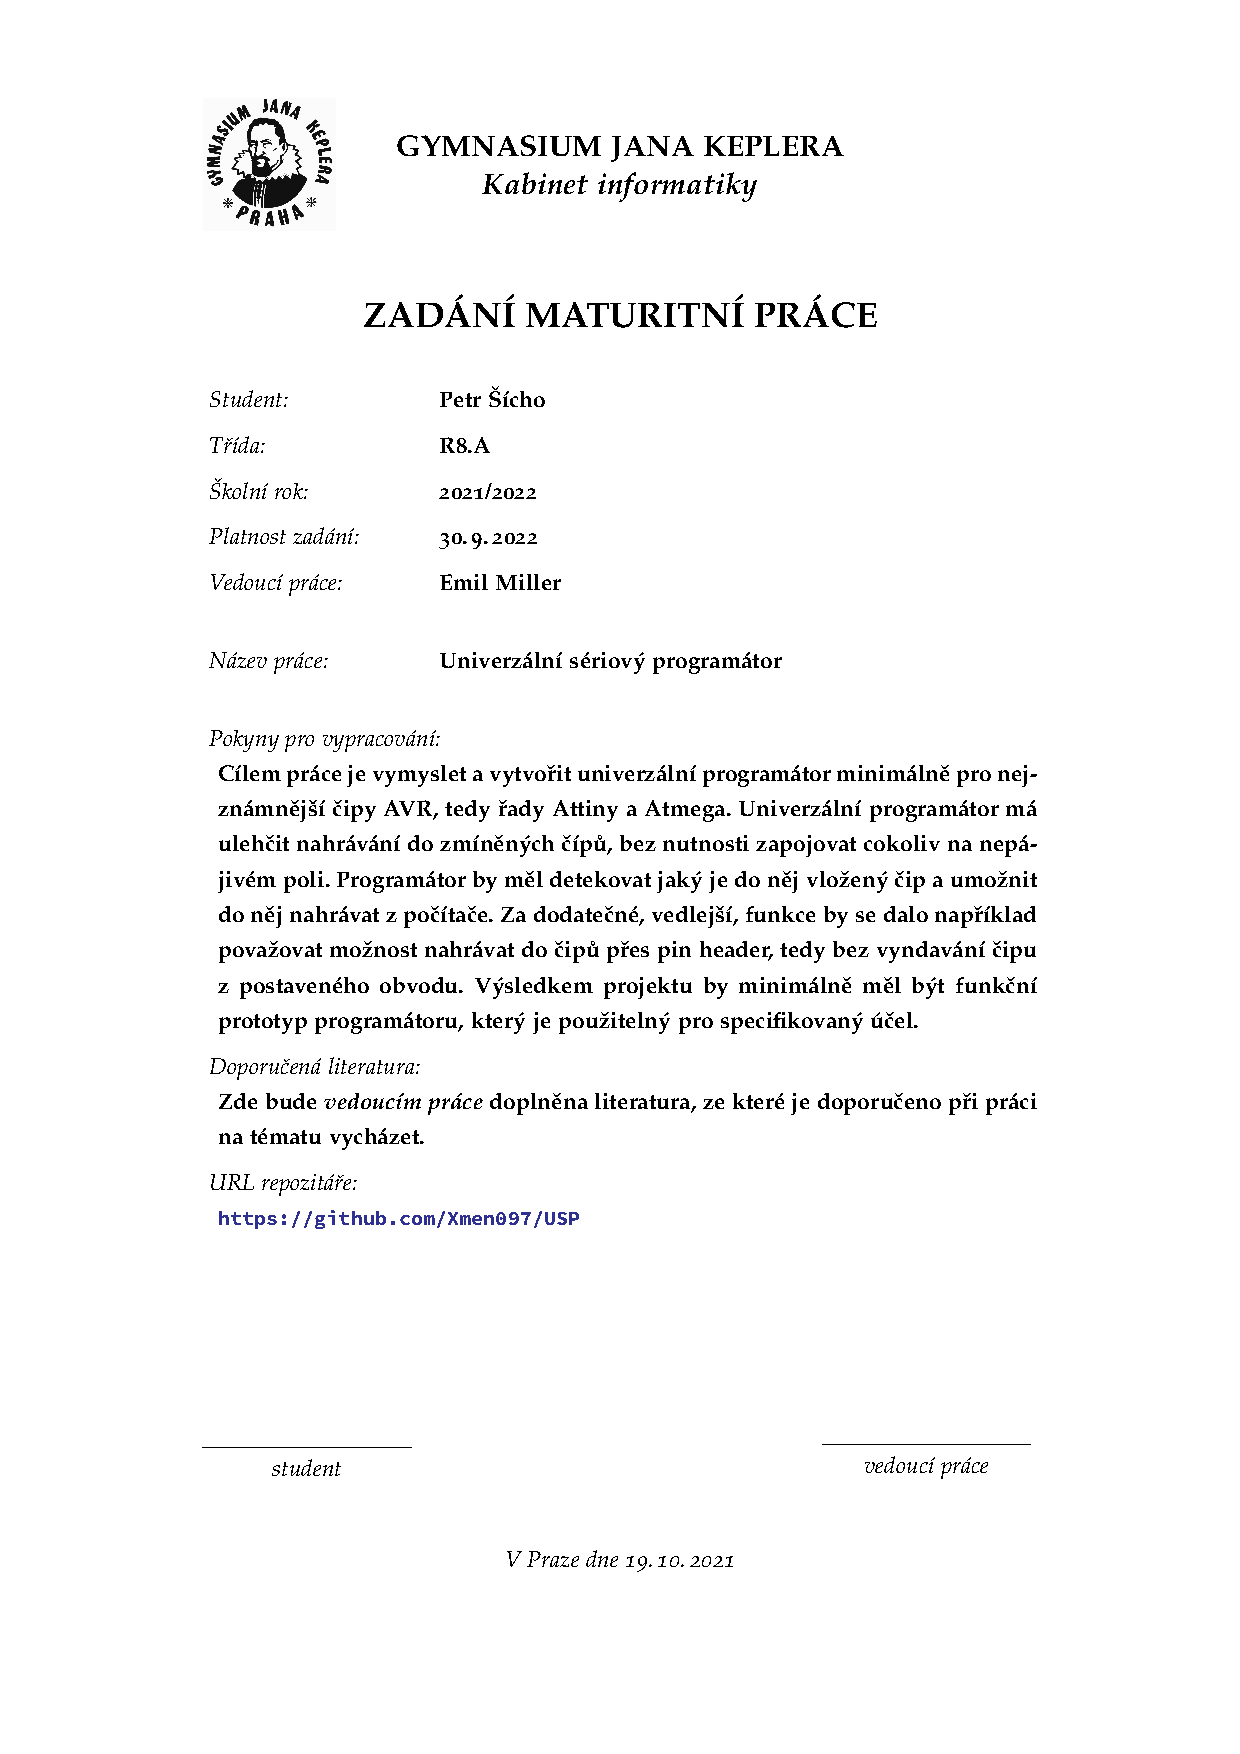
\includepdf[]{zadani.pdf}


%%% Strana s čestným prohlášením k bakalářské práci

\hypersetup{pageanchor=true}
\cleardoublepage
\vspace*{\fill}
\section*{Prohlášení}
\noindent
\Prohlaseni

\vspace{2cm}
\noindent
V Praze dne \today
\hspace*{\fill}\small{\AutorPrace}
\vspace{1cm}

%%% Poděkování
\openright
\vspace*{\fill}
\section*{Poděkování}
\noindent
\Podekovani
\vspace{1cm}


%%% Povinná informační strana bakalářské práce
\openright
\section*{Abstrakt}
\noindent
\Abstrakt
\subsection*{Klíčová slova}
\noindent
\KlicovaSlova

\vfill

\section*{Abstract}
\noindent
\AbstraktEN
\subsection*{Keywords}
\noindent
\KlicovaSlovaEN

\openright
\pagenumbering{arabic}

% Obsah
\setcounter{tocdepth}{2}
\tableofcontents

\chapter{Teoretická část}
\pagestyle{fancy}

Stejně jako existuje nepřeberné množství různých čipů, je také značné množství možných rozložení vývodů, které není jednotné ani u konkrétní velikosti a jednoho výrobce. Pro každé rozložení je nutné mít nebo si postavit externí nahrávací obvod. Cílem USP je sjednotit tyto nahrávací obvody do jednoho univerzálního, který se přizpůsobí vloženému čipu. Programátor má tedy dvě principiální části - detekci a nahrávání. 

Chceme-li vytvořit opravdu univerzální programátor, není možné použít žádný dedikovaný hardware, který by zajišťoval nahrávání. Naopak se nám hodí použít univerzálních vstupních~/~výstupních pinů neboli GPIO pinů \footnote{z anglického General-purpose input/output, tedy pin, který se umí chovat buď jako digitální vstup, nebo výstup, přičemž mezi těmito módy je možné přepínat.}.

Jako minimální požadovanou funkcionalitu jsem bral podporu čipů AVR od výrobce Atmel, konkrétně pak řady ATmegy a ATtiny, které zahrnují čipy, jež pohání známé desky Arduino. Jde o čipy, které jsou oblíbené pro svou jednoduchost a i já je nejčastěji používám. Přestože se snažím o vytvoření univerzálního programátoru, přišlo mi vhodné vzít si určitou rodinu čipů jako referenční bod, neboť nikdy stejně nedocílíme podpory 100\% všech čipů. Na těchto čipech zároveň budu testovat funkce programátoru. Přesto doufám, ikdyž to nemůžu otestovat, že vlastnosti těchto čipů, na kterých je detekce a nahrávání postaveno budou do velké míry přenositelné i na jiné rodiny či výrobce čipů.

\section{Detekce}

Základem detekce je poznat jak velký čip je - tedy kolik má vývodů. Jen díky tomu se nám radikálně sníží počet možných kandidátů. Při zahrnutí jen několika modelů, jednoho pro každou velikost, bychom tak měli prakticky hotovo. Bylo by však nutné arbitrárně stanovit tyto podporované čipy, přičemž při vložení jiného, ať třeba ze stejné rodiny, který má prohozené piny GND a VCC, by došlo pravděpodobně k jeho zničení. Naší ambicí tedy bude zjistit o čipu co nejvíce informací, díky nimž budeme schopni rozeznávat mezi velkým počtem různých čipů.

Při všem musíme dbát, abychom čip nepoškodili. Budeme se snažit držet v hodnotách, které povoluje datasheet. Vzhledem k tomu, že to, o co se pokoušíme není standardní zacházení s čipy, nenalezneme v datasheetu konkrétní povolené hodnoty a situace, kterým můžeme čip bezpečně vystavit. Můžeme z něj ale vyčíst ale základní principy, kterých bychom se měli držet, abychom minimalizovali poškození čipu. Konkrétně se jedná o:
\begin{itemize}
	\item Nevystavovat žádný pin napětí nižšímu než $-0.5V$
	\item Nevystavovat žádný pin, kromě RESETu, napětí vyššímu než ${V}_{cc} + 0.5V$
	\item Nevystavovat RESET napětí vyššímu než $13V$
	\item Nenechat mezi žádný dvěma piny nezapojeného čipu téct nezanedbatelně velký proud po nezanedbatelně dlouhou dobu
\end{itemize}
Při splnění těchto podmínek by měl být čip dostatečně chráněn obvody, které běžně slouží k ochraně proti elektrostatickým výbojům (ESD), které jsou zabudovaná do prakticky všech čipů. \footnote{Pro naše účely budeme považovat za zanedbatelný proud řádu mikroampér a čas mikrosekund.}

\subsection {Detekce velikosti a polohy \label{theory:capacitance}}

Pro detekci velikosti čipu můžeme využít například toho, že každá reálná součástka, kromě svých primárních vlastností, vykazuje také elektrickou kapacitu. To bude jistě platit i pro spoje a součástky uvnitř integrovaných obvodů. Elektrická kapacita pinů jednoduchých CMOS\footnote{Complementary metal-oxide semiconductor; technologie výroby integrovaných obvodů} čipů\cite{multiplexer, switch2, switch1} se pohybuje řádově v hodnotách pikofaradů, což není mnoho. Budeme tedy potřebovat měřit elektrickou kapacitu s dostatečnou přesností. Není mi znám žádný způsob přímého měření elektrické kapacity, budeme tedy muset provést měření nepřímé. Můžeme kapacitor pomalu nabíjet nebo vybíjet a měřit čas, který to zabere. Bude takové měření ale dostatečně přesné? Zkusíme to odhadnout s pomocí rovnice definující energii elektrického kondenzátoru \begin{equation} W = \frac{1}{2}CU^2 \end{equation}
Budeme-li kapacitor nabíjet napětím $U$ a proudem $I$ po dobu $t$, dodáme mu tím maximálně
\begin{equation} {W}_{max} = U \cdot I \cdot t \end{equation} 
Jedná se o horní odhad vykonané práce, která počítá s nulovým odporem kapacitoru a nulovým elektrickým potenciálem kapacitoru. Úpravou vztahů můžeme vyvodit úměrnost
\begin{equation} C \simeq t / R \end{equation}

Kapacita je tedy přímo úměrná času, po který jsme kapacitor nabíjeli a nepřímo úměrná odporu, přes který jsme nabíjeli.\footnote{Ke stejnému výsledku bychom došli i použitím rozměrové analýzy.} Čas budeme schopni měřit velice přesně, nabíjet bude možné po dobu řádově mikrosekund ($10^{-6} s $). Řekněme, že budeme chtít zjistit změnu kapacity $10 pF = 10^{-11} F$. Dosazením do vztahu (1.3) zjistíme, že k tomu budeme potřebovat nabíjecí odpor o velikosti řádově $100 k\Omega$. To vypadá proveditelně.

Změřením kapacity každého z pinů socketu zjistíme nejenom jak velký čip je, ale zároveň s tím určíme kde přesně v socketu je vložen. Není tedy nutné nijak specifikovat kam má být čip pro nahrávání vložen.

\subsection {Detekce speciálních pinů}

Každý mikrokontrolér má kromě vstupně/výstupních pinů i piny, které slouží k nějaké speciální funkci. Například může jít o RESET pin, napájecí piny (GND a VCC) nebo piny hodin (XTAL). Tyto piny budou pravděpodobně vykazovat rozdílné vlastnosti od ostatních pinů. Největší rozdíl bude v napájecích pinech, které jsou vnitřne připojené k všemožným součástem mikrokontroléru. Při dostatečně přesném měření kapacity bychom mohli tyto rozdíly detekovat.

\subsection {Rozpoznání VCC od GND\label{VCCvsGND}}

Při špatném rozpoznání mikrokontroléru může největší poškození způsobit převrácení pinů GND a VCC. Abychom se tomuto problému vyvarovali, bylo by dobré rozpoznávat s jistotou VCC a GND, protože měření kapacity nebude nejspíš dostatečně přesné na jejich rozlišení. 

\begin{figure}[ht!]
  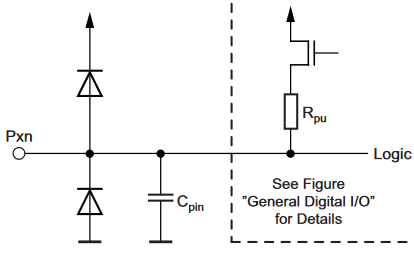
\includegraphics[width=0.4\textwidth]{img/pin_diagram.png}
  \centering
  \caption{Schéma vnitřního zapojení IO pinu mikrokontroléru \cite[str.~58]{atmega328}}
  \label{fig:pin_diagram}
\end{figure}

Využijeme ochranných diod, které jsou připojeny ke každému IO pinu mikrokontroléru jak ukazuje obrázek \ref{fig:pin_diagram}. Povšimněme si, že dioda spojující pin s GND směřuje opačně než dioda spojující pin s VCC. Díky tomu bychom měli být schopni rozpoznat, zda je určitý pin GND či VCC.

Pin GND můžeme detekovat takto. Budeme znát úbytek napětí na diodě $U_d$. Přivedeme-li na pin GND napětí $U$ převyšující $U_d$, měli bychom na všech IO pinech detekovat napětí $U-U_d$. Napětí $V$ by mělo být co nejmenší možné, konkrétně $U<0.5V$. Napětí přivedeme přes dostatečně velký odpor tak, aby mikrokontrolérem a diodou tekl co nejmenší proud. S malým procházejícím proudem budeme mít také menší úbytek napětí na diodě (menší, než běžně udávaný $\sim0.7V$)

Obdobným způsobem je možné detekovat pin VCC. Stačí na libovolný (nebo lépe postupně na všechny) IO pin přivést napětí $U$ a na pinu VCC by se nám vždy mělo ukázat napětí $U-U_d$.

\section {Nahrávání}

Po detekování čipu nám už zbývá pouze do něj nahrát. Vzhledem k tomu, že přesně nevíme jaké rozložení pinů bude čip mít, budeme použít tzv. bit-banging \footnote{Softwarová implementace určitého protokolu, která přímo generuje protokolem specifikovaný signál, bez použití specializovaného hardwaru}. Díky tomu se nemusíme na při stavbě nahrávače na určité čipy, ale bude teoreticky možné nahrávat do všech čipů, které nevyžadují příliš velké komunikační rychlosti. 

Některé programovací protokoly vyžadují použití vyššího napětí. U AVR čipů jde konkrétně o HVSP (high voltage serial programming) a HVPP (high voltage parallel programming), které se hodí při určitém nastavení mikrokontroléru, při kterém není možné standardní programování.\footnote{Jde např. o situace kdy je vypnuté resetování pomocí RESET pinu, protože ho chceme použít na jinou funkci.} Vysokým napětím je v obou případech myšleno 12 voltů.\cite{AVRprog}

\section {Shrnutí požadovaných funkcí\label{pinFunc}}

V této sekci si shrneme funkce, které budeme potřebovat pro úspěšnou detekci a nahrávání do čipů. Tyto funkce by měl mít každý z pinů socketu, neboť nevíme kde zrovna se čip ocitne. Některé funkce budou komplexní (přečti kapacitu připojenou k pinu), u jiných se bude jednat o nějaký elementární stav (připojení k zemi/5V). Některé funkce nebo stavy, které zde budou vyjmenované, třeba bod 1 a 3, se prolínají nebo jsou velmi podobné. Zmiňuji je separátně proto, že jsou potřeba z jiného důvodu a mohly by být implementovány rozdílně.

\begin{enumerate}
\item \textbf{5V s proudem >20 mA} je potřeba pro napájení čipu. Proud 20 mA by měl stačit pro napájení malých AVR čipů.\cite{attiny85} Větší čipy mají sice větší spotřebu než 20 mA, ale mají také několik separátních napájecích pinů, mezi které se proud rozloží.\cite{atmega328}
\item \textbf{0V (GND) s proudem >20 mA} je potřeba též pro napájení čipu. 
\item \textbf{5V s libovolně malým proudem} reprezentuje logický stav 1 při komunikaci, odebíraný proud bude zanedbatelný
\item \textbf{0V (GND) s libovolně malým proudem} reprezentuje logický stav 0 při komunikaci
\item \textbf{Čtení digitální hodnoty} pro čtení odpovědi čipu při nahrávání; standardní funkce GPIO pinů
\item \textbf{Přečtení kapacity} pro detekci čipu
\item \textbf{Napětí přibližně 0.4-0.5V} je potřeba pro rozpoznání GND a VCC, viz sekce \ref{VCCvsGND}
\item \textbf{Přečtení napětí na pinu} je také potřeba pro rozpoznání GND a VCC
\item \textbf{12V} bude potřeba pokud budeme chtít high-voltage programování.
\item \textbf{Nepřipojeno} k ničemu. Piny, které nevyužíváme k jiné funkci by se měly chovat tak, jako kdyby nebyly k ničemu připojení.
\end{enumerate}

\chapter{Implementace}

Implementace projektu měla dvě fáze. Nejprve bylo potřeba navrhnout hardwarovou část - vymyslet a vyzkoušet jednotlivé části obvodu tak, aby plnili požadované funkce. Poté je bylo potřeba všechny spojit do jednoho obvodu, který se vyrobí jako plošný spoj. Po osazení plošného spoje součástkami a otestování základní funkčnosti přišel čas na software. Nejdříve bylo potřeba implementovat low-level komunikaci s jednotlivými součástkami, pak přišly na řadu high-level funkce. Pojďme si jednotlivé fáze rozebrat detailněji.

\section {Hardware}

Převážná část práce na hardwaru probíhala s pomocí nepájivého pole, na kterém jsem postupně testoval jednotlivé ideje uvedené v teoretické části práce. V následujících sekcích detailně popíši jaké součástky byly použity a jak se pomocí nich implementují požadované funkce.

\subsection {Vkládání čipu}

Jako patici, do které se bude vkládat čip k programování jsem zvolil ZIF (zero insertion force) socket. Jak již jméno napovídá, pro vložení čipu do patice není na čip nijak tlačit. Stačí čip položit na patici a pomocí páčky na straně patice se pak čip zajistí a vytvoří se spolehlivý kontakt s piny čipu. Nehrozí tedy ohnutí nožiček čipu a jeho vyndání a zandání je velmi rychlé. Nevýhodou ZIF socketu může být o trochu vyšší pořizovací cena a větší velikost, ale i přesto se v našem případě ZIF socket vyplatí. Konkrétně jsem zvolil patici se 40 piny (dvaceti na každé straně), která by měla postačovat pro naprostou většinu DIP \footnote{Dual in-line package; pouzdro s THT piny s roztečí 2.54mm} pouzder. Patice podporuje vložení jak úzké (0.3''), tak široké (0.6'') varianty DIP.

\subsection {Řídící mikroprocesor}

Bylo potřeba zvolit mikroprocesor, který bude ovládat celý nahrávač. Volil jsem mezi mikrokontroléry AVR, s kterými jsem nejvíce obeznámen, umí jednoduše komunikovat s Arduino IDE a také pro ně existují knihovny, které se nám budou dále hodit. Zásadní otázkou, kterou bylo potřeba vyřešit je počet potřebných GPIO pinů na mikrokontroléru. Budeme potřebovat jeden pin pro každý pin ZIF patice, tedy 40. Další desítky pinů budou potřeba pro ovládaní dalších potřebných komponent, o kterých se budu detailněji zmiňovat v dalších sekcích. Teoreticky by bylo možné přidat další piny pomocí shift registrerů či IO expanderů. Tím by však utrpěla rychlost komunikace a vzrostla by komplexita desky a tím i prostor pro chyby. Rozhodl jsem se tedy pro jeden co největší čip, který bude dostupný. Tím je mikrokontrolér ATmega2560 v pozdře TQFP100, který má 84 GPIO pinů, což by mělo stačit.\cite{atmega2560} 

Nejprve jsem plánoval, že bych využil dostupných schémat Arduino desek a v upravené podobě je přímo zakomponoval do desky nahrávače. To by o něco snížilo náklady na jednu desku, umožnilo využít čip bez omezení. Vzhledem k tomu, že nejsem schopný sám osadit plošný spoj SMD součástkami s tak malými vývody, chtěl jsem si nechat plošný spoj osadit spolu s výrobou. Žádný výrobce nedodává méně než 5 kusů desek, což by znamenalo čtyři zbytečné ATmegy. Proto jsem se rozhodl programátor vyvynout jako shield (nasazovací desku) na Arduino mega ve variantě s procesorem Atmega2560. Nevýhodou tohoto postupu je snad jen to, že Arduino mega dává k dispozici pouze 70 z 84 GPIO pinů, ale i to by mělo pro projekt stačit.\cite{ArduinoMega}

\subsection {Funkcionalita pinů}

Nyní přichází na řadu implementace požadovaných funkcí popsaných v sekci \ref{pinFunc}. Ke každému pinu ZIF socketu bude připojený jeden GPIO pin. Jenom tímto samo o sobě zajistíme funkce 3, 4, 5, které GPIO pin zvládá nativně. Funkce 1 a 2, které vyžadují minimální proud 20 mA také s trochou opatrnosti jednoduše zvládneme. Digitální piny ATmegy2560 dokáží dodávat maximální proud 40 mA \cite[str.~355]{atmega2560}. Musíme tedy jen dát pozor na to, aby další součástky, které budou zapojeny mezi GPIO pinem a pinem ZIF socketu neměly příliš velký odpor nebo nevyžadovaly více omezený protékající proud. S dalšími funkcemi to již nebude tak jednochuché.

Desátý požadavek vyžaduje trochu zamyšlení. Pin určitě nebude možné fyzicky odpojit, to bychom museli provést manuálně. Budeme tedy alespoň chtít maximalizovat odpor čili minimalizovat proud, který může skrz tento \lq odpojený\rq  pin téct. Když nastavíme pin jako vstupní, bude ve stavu s tzv. vysokou impedancí, tedy budou jím téct velmi malý proud. Datasheet specifikuje maximální proud jako $1 \mu  A$, typický proud ale očekávám výrazně menší. Odpojení si navíc můžeme pojistit použitím analogového přepínače, u kterého je udáván maximální proud $100nA$ a typický $0.05nA$.\cite[str.~3]{switch1}

\subsubsection {Zapojení multiplexerů}

Implementaci funkcí 6, 7, 8 a 9 si zjednodušíme pozorováním, že v jednu chvíli bude daná funkce potřebná pouze na jednom pinu. Nemusíme ji tedy implementovat 40x, ale můžeme použít multiplexery k spojení určitého pinu s požadovaným stavem nebo obvodem zajišťujícím funkcí. Napětí na pinu budem číst pomocí ADC\footnote{Analogově digitální převodník; zařízení, které převede analogový signál (napětí) v určitém rozsahu na digitální tvar s určitým počtem bitů, v našem případě se jedná o převodník 10-bitový} převodníku. Atmega2560 disponuje jedním ADC převodníkem, který je ale vnitřne multiplexován na 16 různých pinů. My dále pomocí multiplexerů rozšíříme tuto funkcionalitu na všech 40 pinů.

Pro zajištění správného přečtení napětí nemůžeme nechat ADC převodník tzv. floating, tedy nepřipojený k ničemu, kdy vrací víceméně náhodné hodnoty. ADC pin jsem tedy připojil rezistorem $1M\Omega$ k zemi. Takto vysokou hodnotu rezistoru jsem volil, abych nezkreslil měření kapacity.

Multiplexery se standardně vyrábí s $2^n$ kanály, které se ovládají pomocí $n$ pinů. Zvolil jsem 8 kanálové multiplexery\cite{multiplexer}, tedy s 3 ovládacími piny. Pro obsluhu 40 pinů jich bude potřeba celkem 5. Multiplexery jsou připojeny k pinům ZIF socketu způsobem znázorněným na obrázku \ref{fig:mux_diagram}

\begin{figure}[ht!]
  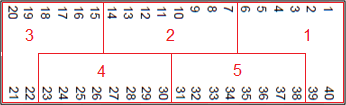
\includegraphics[width=0.4\textwidth]{img/mux_diagram.png}
  \centering
  \caption{Schéma zapojení mulitplexerů k pinům ZIF patice}
  \label{fig:mux_diagram}
\end{figure}

Díky tomuto způsobu zapojení budeme schopni odhalit závadu na multiplexeru při rozpoznávání čipu, neboť i nejmenší čip, který má pouzdro DIP4 se 4 piny na každé straně bude vždycky mít alespoň dva piny v různých multiplexerech. Nestane se tedy, že by kvůli závadě na jednom multiplexeru (ta může být způsobená i třeba dotekem uživatele, čímž se zvýší kapacita) byl čip chybně rozpoznán.

\subsubsection {Napěťový dělič}

Napětí 0.4-0.5V, jak si žádá 7. požadavek, vytvoříme pomocí napěťového děliče. Zde se nám budou hodit již výše zmíněné multiplexery. Dělič napětí totiž vytvoříme právě mezi GPIO pinem a multiplexovaným pinem. Na každém GPIO pinu je možné zapnout tzv. pullup rezistor, který pin připojí přes odpor s přibližnou velikostí $30-40k\Omega$\footnote{Datasheet udává, že odpor bude vždy větší než $20k\Omega$ a menší než $50k\Omega$. Vzhledem k tomu, že tyto hodnoty jsou pro teplotní rozmezí od -55°C do 125°C můžeme konstatovat, že při pokojové teplotě bude odpor přibližně mezi $30-40k\Omega$.} k 5 voltům. Chtěné napětí přibližně půl voltu vytvoříme dalším rezistorem s velikostí $3300\Omega$\footnote{Chceme dělič napětí přibližně 1:10, hodnotu odporu jsem zvolil spíše o něco nižší, protože i samotný multiplexer bude mít určitý odpor (asi 100 ohmů).} k zemi. Zapojení děliče napětí na pinu je vidět na obrázku \ref{fig:voltage_divider}


\begin{figure}[ht!]
  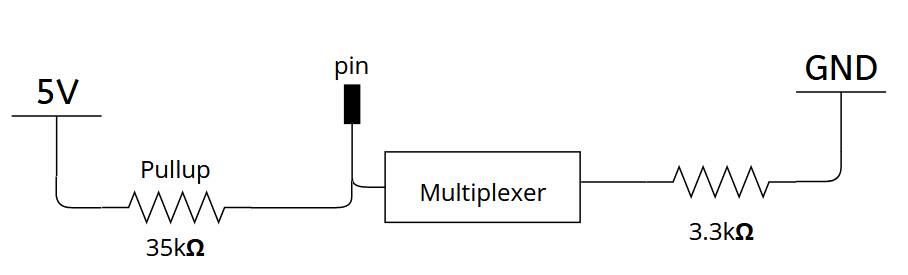
\includegraphics[width=0.6\textwidth]{img/voltage_divider.png}
  \centering
  \caption{Schéma děliče napětí na pinu}
  \label{fig:voltage_divider}
\end{figure}

\subsubsection{Měření kapacity}

Kapacita lze měřit, jak jsme vyvodili v sekci \ref{theory:capacitance}, pomocí pomalého nabíjení - tedy nabíjení přes dostatečně velký rezistor. Vypočítali jsme sice, že by se nám hodil rezistor s odporem $100k\Omega$. Připojovat takový odpor k pinům by si vyžádalo dalších multiplexerů nebo switchů. Můžeme ale využít stejných pullup rezistorů, které využíváme pro napěťový dělič. Ty jsou o něco menší a mohlo by se stát, že kapacitor nabijeme příliš rychle. Můžeme ale chytře využít ADC převodníku, který máme multiplexovaný k pinům. Původně jsme chtěli měřit čas, za který nabijeme plně kapacitor, což bychom zjišťovali pomocí digitálního vstupu GPIO pinů. Můžeme to ale provést i opačně. Kapacitor budeme nabíjet nějaký konstantní čas, a poté pomocí ADC převodníku zjistíme napětí na kapacitoru. Čím vyšší napětí bude, tím více jsme kapacitor nabili a tím je tedy kapacitor menší. Další možností by bylo kapacitor plně nabít a přestat ho nabíjet, čímž se začně postupně vybíjet. Počkáme konstantní čas a opět pomocí ADC převodníku zjistit jak moc se vybil. 

Při testování ukázalo se dokonce ukázalo, že pro měření kapacity se nám velmi hodí i dělič napětí, více o tom však až v sekci \ref{software:capacitance}

\subsubsection {Napětí 12 voltů}

Poslední funkcionalitou, kterou nám zbývá implementovat je dostupnost napětí 12 voltů. Ty bychom na pin pouštěli pomocí stejných multiplexerů, které využíváme k připojení ADC převodníku. Stačí pomocí switche\cite{switch2} přepínat zdroj multiplexeru mezi 12 volty a ADC převodníkem. Zapojení tohoto obvodu pro multiplexer 1 a 2 je vyobrazeno v příloze č. \ref{appendix:mux_input_control}. Od použitého switche nepožadujeme žádné zvýšené nároky ohledně proudu, pro HVSP i HVPP nám stačí libovolně malý proud. Obecně se ale ukázalo, že podpora 12 voltů nám celou situaci značně zkomplikuje. Náš řídící mikrokontrolér, ale ani většina dobře dostupných multiplexerů nepodporuje vyšší napětí než 5 voltů. S trochou snahy se dají najít i multiplexery podporující 12 voltů. Řídíci čip jehož piny odolají napětí 12 voltů ale prakticky možné není. Budeme proto muset piny řídíciho mikrokontroléru v případě připojení 12 voltů odpojit. K tomu využijeme analogové switche\cite{switch1}. Vzhledem k tomu, že přes tyto switche budeme mimo jiné napájet čip, který budeme chtít programovat, musí podporovat průtok proudu alespoň $20mA$.\footnote{Z tohoto důvodu se použitý switch liší od switchů \cite{switch2}, které používáme u zdroje multiplexeru.} Každý switch má 4 kanály, které dokáže přepínat a k tomu používá 4 ovládací piny. Není možné ani potřebné ovládat každý z těchto ovládacích pinů individuálně, na to bychom totiž spotřebovali dalších 40 pinů.

Uvažoval jsem dvě možnosti. Šlo by pomocí tranzistorů a odporů detekovat zvýšené napětí a přepnout ovládací pin switche. To by však vyžadovalo značné množstí externích komponent - na každý pin jeden tranzistor a několik odporů. Lepší řešení je založené na faktu, že 12 voltů bude vždy připojené na pinu, který je multiplexován. Toho využijeme a přidáme další multiplexer, který bude mít stejně zapojené ovládací piny jako první multiplexer. Jeho funkce bude, že vypne switch, který obsluhuje pin, ke kterému je multiplexováno. Tímto zajistíme přepínání s použitím pouze jediného pinu, který bude sloužit k potlačení této funkcionality, která by nám v opačném případě rozbila napětový dělič a další funkce. Zjednodušené schéma tohoto systému pro 8 pinů je znázorněno na obrázku \ref{fig:simplified_pin_switches}. Tento obvod je na USP celkem 5 krát - pro každých 8 pinů, a to podle stejné schématu jako zapojení původních multiplexerů (obrázek \ref{fig:mux_diagram}). Kompletní zapojení toho obvodu je dostupné jako příloha č.\ref{appendix:pin_switches}

\begin{figure}[ht!]
  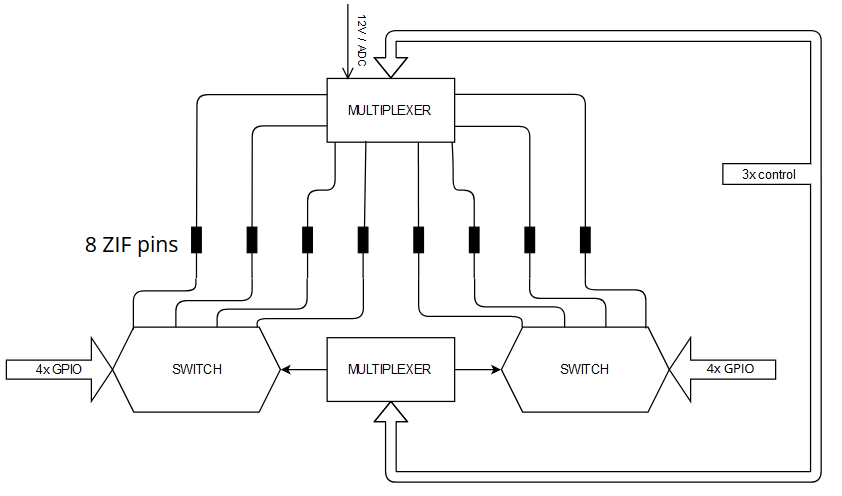
\includegraphics[width=0.8\textwidth]{img/simplified_pin_switches.png}
  \centering
  \caption{Zjednodušené schéma obvodu připojeného k 8 pinům ZIF patice}
  \label{fig:simplified_pin_switches}
\end{figure}

Další kompilkací, kterou vyšší napětí přineslo bylo to, že multiplexery a switche potřebují být ovládané tímto napětím. Nestačí tedy již připojit na ovládací pin multiplexeru/switche GPIO pin řídícího mikrokontroléru, ale je nutné použít tranzistor a pullup/pulldown\footnote{V závislosti na tom v jakém výchozím stavu chceme, aby byl ovládací pin; ve většine případu se bude jednat o pulldown rezistor} rezistor.

Poslední věcí, kterou musíme vyřešit je kde vůbec získat napětí 12 voltů. Jednou možností by bylo zapojit do zařízení přímo toto napětí z externího zdroje. To by ale výrazně ztížilo použití výsledného zařízení. Rozhodl jsem se proto zabudouvat přímo do USP step-up převodník, který nám vytvoří napětí 12V. Obvod step-up převodníku jsem navrhl podle datasheetu regulátoru\cite{step-up}. Zapojení obvodu převodníku je zobrazeno v příloze č.\ref{appendix:boost_converter}

\subsection {Dodatečný hardware}

Krom výše uvedených součástek a obvodů, které slouží k zajištění detekce nebo nahrávání je USP vybaven také 0.91'' OLED displayem a 4 tlačítky. To umožní tvorbu uživatelského rozhraní pro jednodušší ovládání programátoru. OLED display byl také skvělým nástrojem pro debugování, protože na něm šlo jednoduše zobrazit v reálném čase informace, bez nutnosti komunikace s počítačem přes sériovou linku (která byla potřeba k jiným účelům). Dále jsou pak na programátoru tři LED - modrá, zelená a červená, které slouží pro grafickou signalizaci stavu programátoru.

\subsection {Plošný spoj}

Po otestování částí některých výše zmíněných obvodů na nepájivém poli jsem se pustil do návrhu plošného spoje. První bylo potřeba vytvořit diagramy všech potřebných obvodů a zapojení, část z nich je možné vidět v přílohách č. \ref{appendix:pin_switches}, \ref{appendix:mux_input_control} a \ref{appendix:boost_converter}. Poté přišlo na řadu návrh plošného spoje, kde, vzhledem k tomu, že autorouter\footnote{Program, který má automaticky nalézt a zapojit potřebné spoje na desce} stále moc nefunguje, bylo potřeba \lq natahat \rq cestičky mezi součástkami. Rozhodl jsem se rovnou pro 4-vrstvý plošný spoj, vzhledem k tomu, že jsem plánoval natěsnat co nejvíce součástek na co nejmenší plochu a vrchní vrstva je tak prakticky celá pokryta ploškami pro kontakty součástek. Prostřední dvě vrstvy jsou udělány jako tzv. plane, kdy většina vrstvy zabírá jeden signál, zde konkrétně země a napájení, a slouží pro snížení rušení na desce. Obrázek hotového zapojení plošného spoje v příloze č.\ref{appendix:board}.

Plošný jsou jsem si nechal vyrobit a osadit SMD součástkami u nejmenované čínské firmy. Hlavní výhodou objednání z Číny je řádově menší cena, než u ostatních výrobců, problémem na druhou stranu může být, že čínané mají často vlastní kopie součástek a jejich datasheety nejsou přeložené do angličtiny. Většinou jsou k nalezení anglické datasheety prakticky totožných součástek jiných výrobců. Po výrobení plošného spoje jsem začal zjišťovat na co vše jsem při návrhu zapomenul a co nefunguje. Naštěstí nic z toho nebylo kritické a bylo možné všechny nedostatky opravit.

\section {Software}

\subsection {Nízkoúrovňové funkce}

Jako první bylo na

\subsection {Čtení kapacity \label{software:capacitance}}

\chapter{Technická dokumentace}

Poslední kapitola obsahuje informace o tom, jak projekt, který v rámci maturitní práce vznikl, nainstalovat, spustit a používat.

\chapter*{Závěr}
\pagestyle{empty}
\addcontentsline{toc}{chapter}{Závěr}

Závěr obsahuje shrnutí práce a vyjadřuje se k míře splnění jejího zadání. Dále by se zde mělo objevit sebehodnocení studenta a informace o tom, co nového se naučil a jak vnímal svou práci na projektu.

%%% Seznam použité literatury
\printbibliography[title={Seznam použité literatury},heading={bibintoc}]

%%% Seznam obrázků
\openright
\listoffigures
\addcontentsline{toc}{chapter}{Seznam obrázků}

%%% Seznam tabulek
\clearpage
\listoftables
\addcontentsline{toc}{chapter}{Seznam tabulek}

%%% Přílohy k práci, existují-li. Každá příloha musí být alespoň jednou
%%% odkazována z vlastního textu práce. Přílohy se číslují.

\part*{Přílohy}
\appendix


\begin{figure}[ht!]
  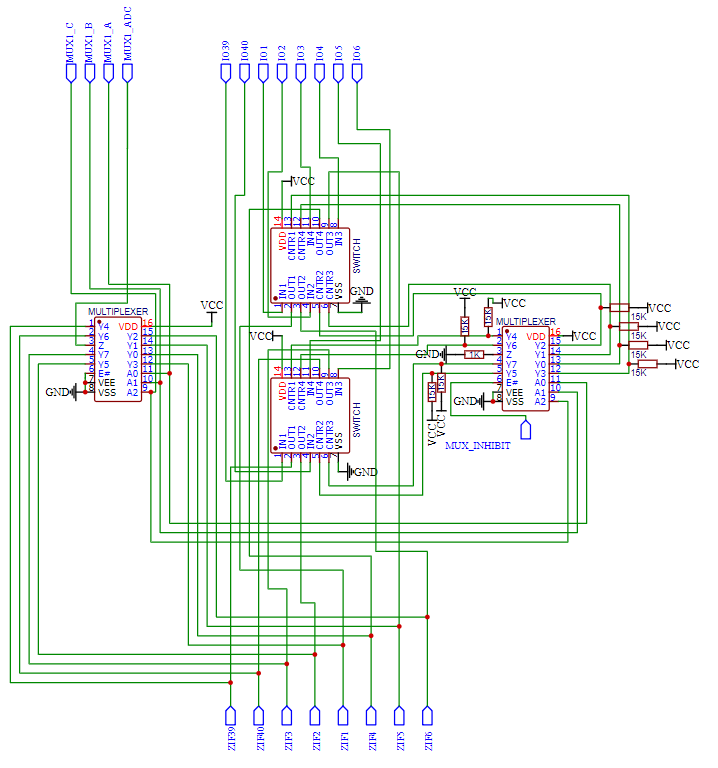
\includegraphics[width=\linewidth]{img/pin_switches.png}
  \centering
  \caption{Úplné schéma obvodu připojeného k 8 pinům ZIF patice}
  \label{appendix:pin_switches}
\end{figure}

\begin{figure}[ht!]
  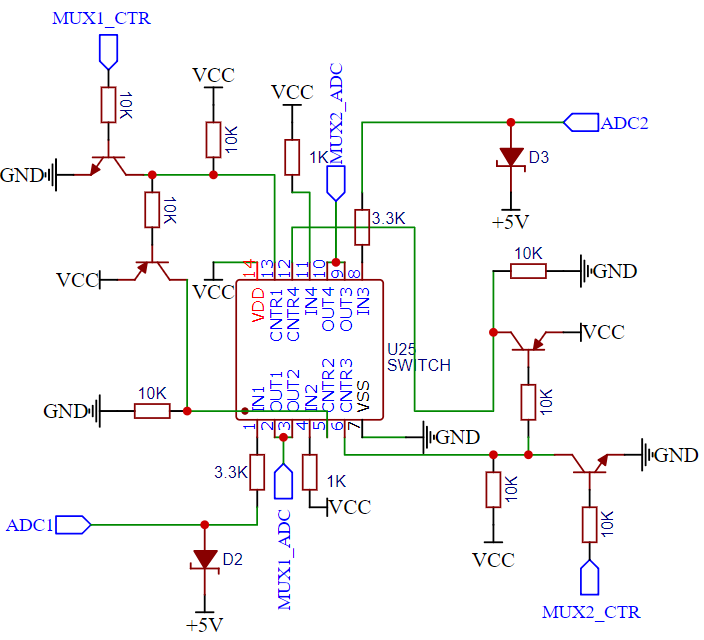
\includegraphics[width=\linewidth]{img/mux_input_control.png}
  \centering
  \caption{Úplné schéma zapojení switche, který přepíná vstup do multiplexerů 1 a 2 mezi ADC pinem a 12V.}
  \label{appendix:mux_input_control}
\end{figure}

\begin{figure}[ht!]
  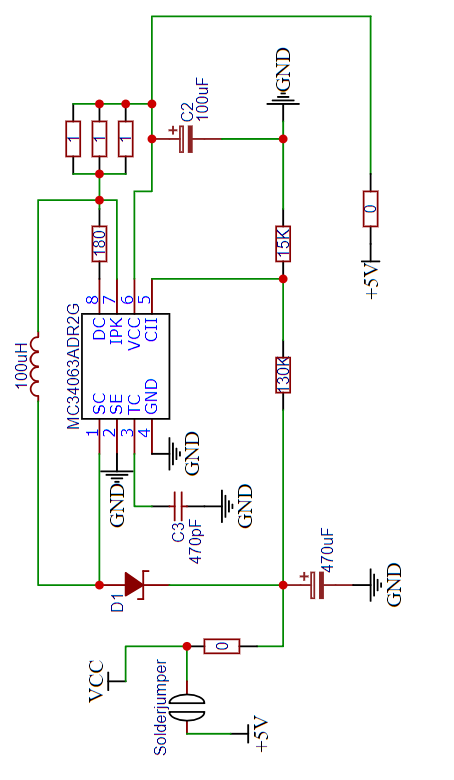
\includegraphics[width=0.8\linewidth]{img/boost_converter.png}
  \centering
  \caption{Úplné schéma obvodu step-up převodníku z 5 na 12 voltů. Obvod zahrnuje 0 ohmové odpory a solder jumper, které umožňují jednoduché odpojení převodníku.}
  \label{appendix:boost_converter}
\end{figure}

\begin{figure}[ht!]
  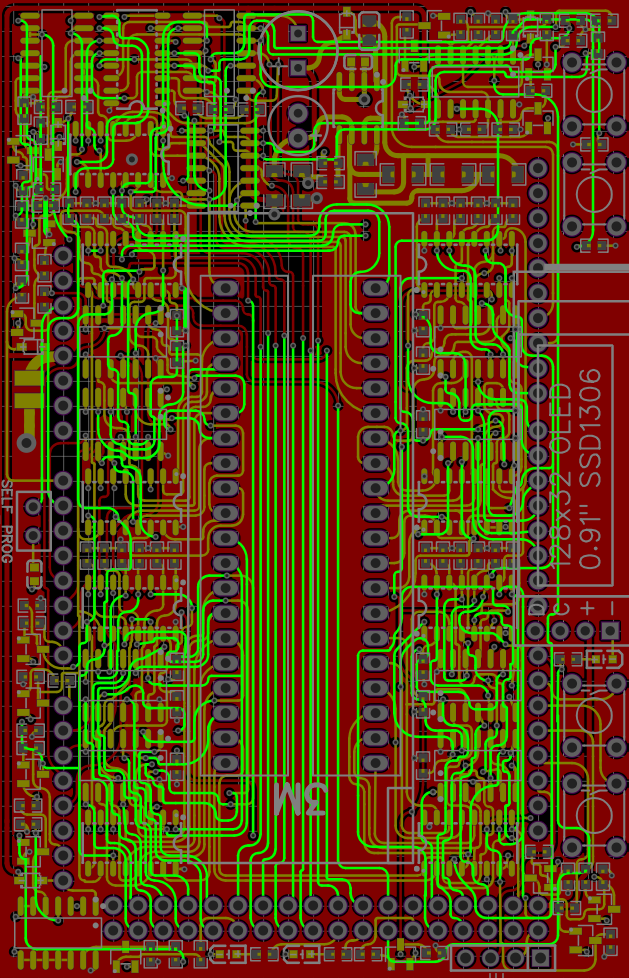
\includegraphics[width=\linewidth]{img/board.png}
  \centering
  \caption{Zapojení plošného spoje. Žludou barvou jsou vyznačeny spoje ve vrchní vrstvě, zelenou spoje spodní vrstvy a červenou spoje jedné z vnitřních vrstev. Druhá vnitřní vrstva není na obrázku zachycena.}
  \label{appendix:board}
\end{figure}

\end{document}
